%% IMPORTANT: Once working, run latex 3 times to get listoffigures to work

%% Be sure to check spelling!

%% Put your name and the proper due date in place

%% Copy the lstinputlisting and figure code as many times as you need
%% Be sure to put in your own file names if appropriate

%% Note that the \epsfig and \lstinputlisting commands 
%% are currently commented out with %%% - until the
%% files exist, processing this code without them will result in an error
%% so leave the comments until you have created the files!

%%% Items starting with %%% are actionable items

\documentclass{article}
\usepackage{amsmath}    % loads AMS-Math package
\usepackage{epsfig}     % allows PostScript files
\usepackage{listings}   % allows lstlisting environment
\usepackage{moreverb}   % allows listinginput environment
\usepackage[letterpaper, margin=0.75in]{geometry}  % set paper size/margins
\usepackage{EGR103F19}  % colorful file imports

\begin{document}
\begin{center}
\rule{6.5in}{0.5mm}\\~\\
\textbf{\large EGR 103L -- Fall 2019}\\~\\
\textbf{\huge Structured Programming I}\\~\\
***Marcus Deans (md374)***\\
***Lab Section 2, Tuesdays 11:45-2:35***\\
***29 September 2019***\\~\\
{\small I understand and have adhered to all the tenets of the Duke
  Community Standard in completing every part of this assignment.  I
  understand that a violation of any part of the Standard on any part
  of this assignment can result in failure of this assignment, failure
  of this course, and/or suspension from Duke University.} 
\rule{6.5in}{0.5mm}\\
\end{center}
\tableofcontents
\listoffigures
\pagebreak

\section{Sinusoids}
%%% Discussion
The $A$ value represents the amplitude of the cosine function. The $A$ value of 2 results in a amplitude twice that of the function with a $A$ value of 1; in this case, the amplitude is precisely two. Conversely, a $A$ value $<1$ would result in a decreased amplitude. The $\omega$ value affects the period of graph by changing the horizontal extension/compression of the graph. As the $\omega$ value increases, the period will decrease as related by the equation $period = ((2\pi)/\omega)$. The $\phi$ value represents the phase shift, or horizontal translation, of the cosine function, thus shifting the function either in the $+x$ or $-x$ direction or ''left or right''. Notably, a positive $\phi$ value will result into a shift to the left, thus perceived as moving in the negative direction, unlike other function transformations.

\section{P\&E 4.48}
%%% Comment out the command below when ready
\lstinputlisting{table_log.txt}

\section{P\&E 2.38}
%%% Comment out the command below when ready
\lstinputlisting{digit_diary.txt}

\section{Chapra Problem 3.10}
%%% Replace the spaces (~) belowwith the appropriate numbers
\begin{itemize}
\item max\_pos\_disp = 1.9532e+02
\item max\_pos\_disp\_loc = 5.7019 ft
\item max\_neg\_disp = =3.2741e+01
\item max\_neg\_disp\_loc = 8.7076 ft
\end{itemize}

\section{Geometric Progression}
%%% Comment out the command below when ready
\lstinputlisting{geo_diary.txt}

\pagebreak
\appendix
\section{Codes}
% Put the name of your file in the subsection name 
% and the lstinputlisting - note that _ need to be \_ in 
% subsection name but not in lstinpustlisting name!

% Be sure to include the community standard in codes!

% Add \pagebreaks if they make sense


% Set default to python
\lstset{style=python103, language=python} 

%%% Copy this as many times as needed for your files;
%%% Remove %%% from lstinputlisting when ready
%%% Note required \_ in subsection name versus _ in file name.

\subsection{Sinusoidal\_.py}
\lstinputlisting{sinusoidal.py}
\clearpage
\subsection{P\&E 4.48\_.py}
\lstinputlisting{multialter3.py}
\clearpage
\subsection{P\&E 2.38\_.py}
\lstinputlisting{alpha.py}
\clearpage
\subsection{Chapra Problem 3.10\_.py}
\lstinputlisting{singularity.py}
\clearpage
\subsection{Geocode\_.py}
\lstinputlisting{finalgeo.py}

%\subsection{FILE\_NAME.py}
%\lstinputlisting{FILE_NAME.py}

\clearpage % start Figures on new page

\section{Figures}
% Remove %%% when ready; use your file names if different from mine
\begin{figure}[ht!]
\begin{center}
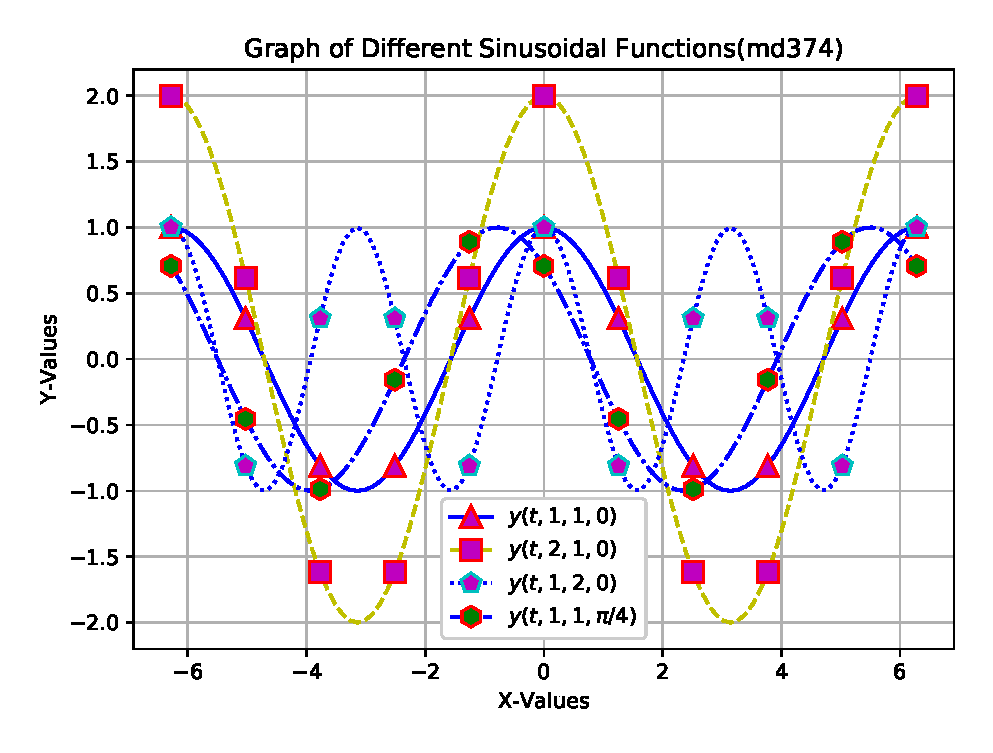
\epsfig{file=sine_plot.eps, width=5in}
\caption{Four sinusoids.}
\end{center}
\end{figure}

\begin{figure}[ht!]
\begin{center}
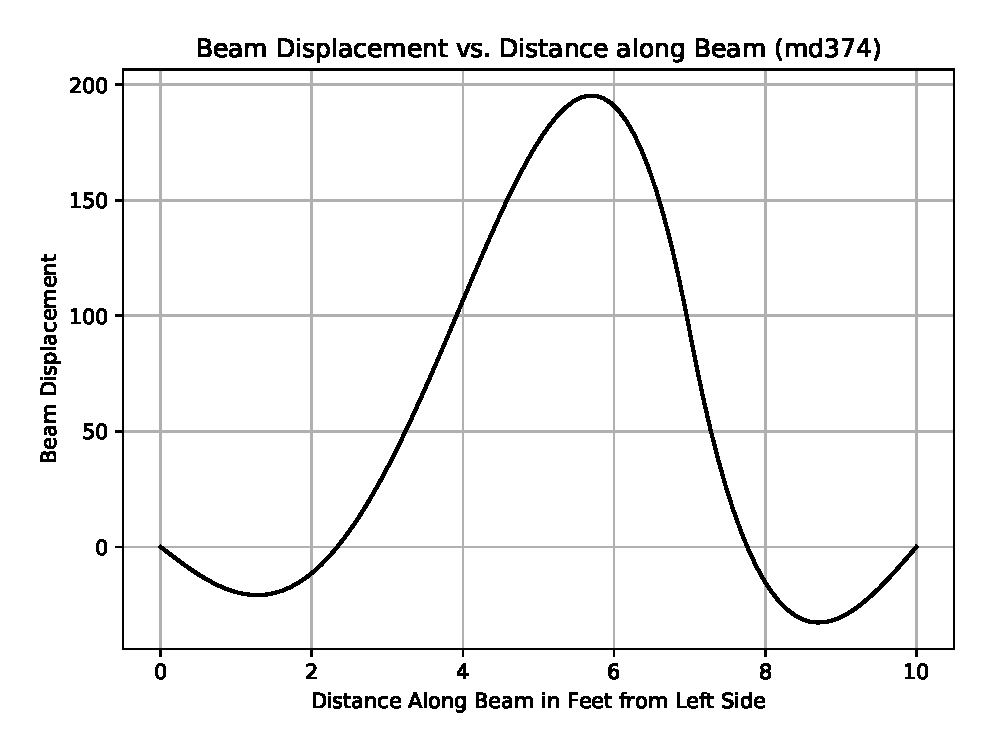
\epsfig{file=SingPlots.eps, width=5in}
\caption{Displacement plot for a beam.}
\end{center}
\end{figure}

\end{document}
